\section{Mexican Grand Prix}

\subsection{Circuit Analysis}

\textbf{Circuit Name:} Autódromo Hermanos Rodríguez (Mexico City, Mexico) \\
\textbf{Length:} 4.304 km - \textbf{Laps:} 71 - \textbf{Total Distance:} 305.354 km

\begin{figure}[H]
    \centering
    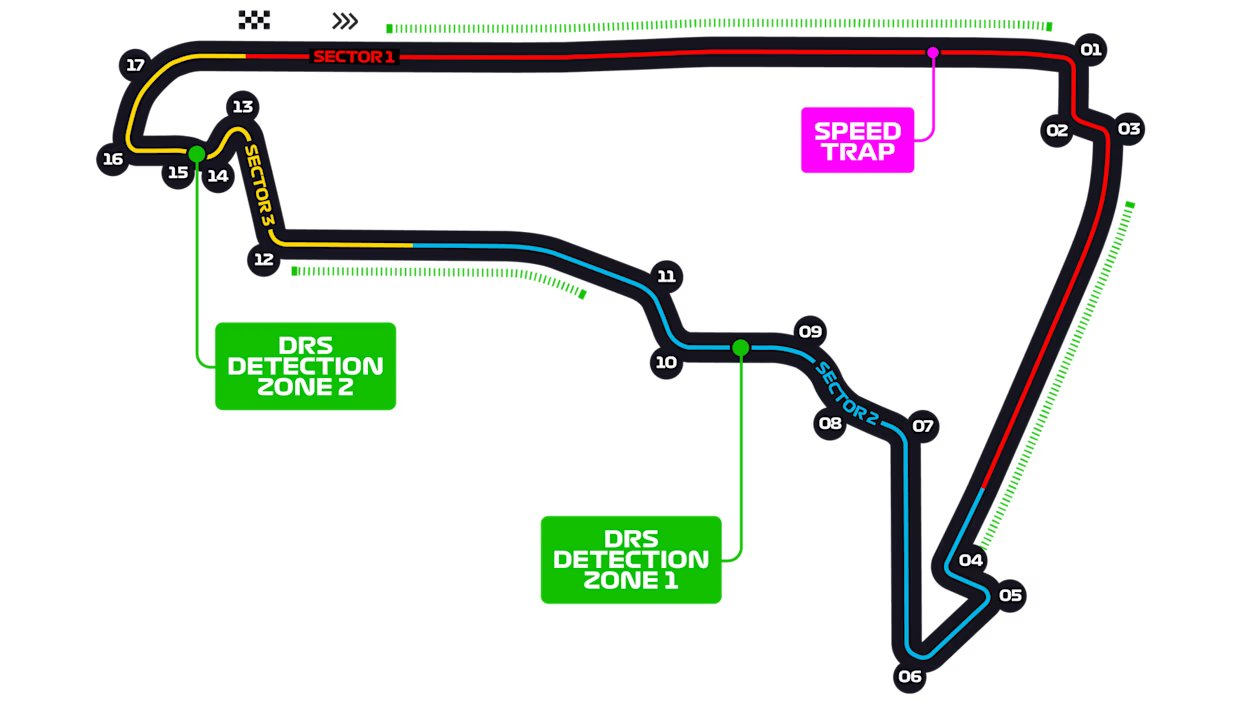
\includegraphics[width=0.75\linewidth]{images/20.Mexico_Circuit.jpg}
\end{figure}

\begin{itemize}
    \item \textbf{Lap Record} : 1:14.758 (2019, Max Verstappen - Red Bull).
    
    \item \textbf{Number of Corners \& Key Features} : 17 turns (10 right, 7 left), mix of long straights and tight technical complexes. \\
    Iconic sections include the long main straight (1.2 km) into Turn 1, and the stadium sector (Turns 12–16) with spectacular crowd atmosphere.
    
    \item \textbf{Braking Zones \& Traction} : Heavy braking into Turn 1 (from 350 km/h to 100 km/h). \\
    Traction critical out of slow corners in the stadium, especially Turn 16 onto the straight.
    
    \item \textbf{DRS \& Overtaking} : Three DRS zones (main straight, between Turns 3–4, and between Turns 11–12). \\
    Turn 1 is the prime overtaking spot, stadium sector allows close racing but little passing.
    
    \item \textbf{Tyre Degradation \& Strategy} : Medium to high wear due to low air density and limited cooling. \\
    Two-stop strategies typical, undercut powerful with long pit lane loss.
    
    \item \textbf{Weather \& Environment} : High altitude (2,240m) reduces engine power and cooling efficiency. \\
    Brakes and tyres face added stress from thin air.
\end{itemize}

\textbf{Strategic Summary :} Mexico demands power unit efficiency under high altitude, strong braking for Turn 1, and tyre management under thermal stress. Track position at the start is crucial due to the long run into Turn 1.

\subsection{Race Analysis}

\textbf{Date:} 27 October 2024 — 14:00 local time 

\begin{itemize}
    \item \textbf{Qualifying Summary} : \textbf{Pole Position:} Carlos Sainz (Ferrari) – 1:15.946. \\
    Grid : Verstappen 2nd, Norris 3rd, Leclerc 4th. \\
    Magnussen P7, Gasly P8 (second consecutive Q3). Piastri and Pérez eliminated in Q1.
    
    \item \textbf{Race Summary} : \textbf{Winner:} Carlos Sainz (Ferrari) — dominant recovery after early loss of lead. \\
    \textbf{Podium:} 1. Sainz - 2. Norris - 3. Leclerc. \\
    Verstappen led the opening laps but penalised twice (20s total) for forcing Norris off track. \\
    Leclerc secured fastest lap on final lap. Hamilton beat Russell for P4 in late Mercedes duel. \\
    
    \item \textbf{Notable Incidents} : \\
    - Lap 1: Gasly causes contact between Tsunoda and Albon → Safety Car. Albon + Tsunoda retire. \\
    - Verstappen penalised (10s for Turn 4 squeeze, 10s for Turn 8 move vs Norris). \\
    - Lap 63: Leclerc slides wide at final corner, Norris overtakes for P2. \\
    - Alonso retires (brakes). \\
    - Colapinto penalised for contact with Lawson. \\
    - Pérez penalised for incorrect grid position.
    
    \item \textbf{Strategies} : \\
    - Sainz: medium → hard (lap 25), fastest overall management. \\
    - Norris: medium → hard, pressured Leclerc late and seized P2 after his error. \\
    - Leclerc: medium → hard, strong but lost P2 under pressure. \\
    - Verstappen: early stop to serve penalty, dropped to P15, recovered only to P6. \\
    - Mercedes: medium → hard, close intra-team battle, Hamilton prevailed. \\
    - Haas: strong pace all weekend, Magnussen P7, Hülkenberg P9. \\
    - Piastri: started P17, recovered to P8 with aggressive stints.
    
    \item \textbf{Performance Trends} : \textbf{Ferrari} fastest overall (pole + win + fastest lap). \\
    \textbf{McLaren} competitive but lacked straight-line defence, Norris maximised recovery. \\
    \textbf{Red Bull} inconsistent, Verstappen’s penalties costly, Pérez invisible at home GP. \\
    \textbf{Mercedes} strong in race pace, but behind Ferrari/McLaren.
    
    \item \textbf{Championship Impact} : \textbf{Drivers:} Verstappen 362 pts, Norris 315, Leclerc 291. \\
    \textbf{Constructors:} McLaren 566, Ferrari 537 (+1), Red Bull 512 (-1), Mercedes 366.
\end{itemize}

\textbf{Key Takeaway :} Carlos Sainz controlled Mexico with Ferrari’s superior pace, while Verstappen’s penalties exposed Red Bull’s growing weaknesses. Norris capitalised late for P2, Leclerc salvaged P3 + fastest lap, and Mercedes showed solid but unspectacular form. Haas confirmed progress with both cars in points.

\subsection{Link \& Takeaway}

\begin{itemize}
    \item Mexico’s long run to Turn 1 reshaped the race start — Verstappen briefly led but couldn’t contain Ferrari’s pace. 
    \item Ferrari’s strength in medium-to-hard stints secured victory, Sainz maximised track position and tyre life. 
    \item Verstappen’s aggressive defence and penalties symbolised Red Bull’s desperation under pressure. 
    \item Norris showed McLaren’s persistence with a late overtake on Leclerc, but Ferrari clearly had the upper hand. 
    \item High altitude punished power units and cooling, teams with efficient aero and tyre control thrived, notably Ferrari and Haas. 
    \item With this win, Ferrari reignited the constructors’ title fight, closing the gap to McLaren and Red Bull with just four races left.
\end{itemize}
